\documentclass[10pt]{article}
\usepackage{picinpar,graphicx,bm}
\usepackage[UTF8]{ctex}
\usepackage{booktabs}
\usepackage{diagbox}
\usepackage{subfigure}
\usepackage{float}
\usepackage{cases}
\usepackage{multirow}
\usepackage{booktabs}
\newcommand{\upcite}[1]{\textsuperscript{\textsuperscript{\cite{#1}}}}


\usepackage{bbding}
\usepackage{pifont}
\usepackage{wasysym}
\usepackage{amssymb}
\usepackage{threeparttable}


\usepackage{listings}
\usepackage{xcolor}
% 定义可能使用到的颜色
\definecolor{CPPLight}  {HTML} {686868}
\definecolor{CPPSteel}  {HTML} {888888}
\definecolor{CPPDark}   {HTML} {262626}
\definecolor{CPPBlue}   {HTML} {4172A3}
\definecolor{CPPGreen}  {HTML} {487818}
\definecolor{CPPBrown}  {HTML} {A07040}
\definecolor{CPPRed}    {HTML} {AD4D3A}
\definecolor{CPPViolet} {HTML} {7040A0}
\definecolor{CPPGray}  {HTML} {B8B8B8}
\lstset{
    columns=fixed,    
   % numbers=left,                                        % 在左侧显示行号
    frame=none,                                          % 不显示背景边框
    backgroundcolor=\color[RGB]{245,245,244},            % 设定背景颜色
    keywordstyle=\color[RGB]{40,40,255},                 % 设定关键字颜色
    numberstyle=\footnotesize\color{darkgray},           % 设定行号格式
    commentstyle=\it\color[RGB]{0,96,96},                % 设置代码注释的格式
    stringstyle=\rmfamily\slshape\color[RGB]{128,0,0},   % 设置字符串格式
    showstringspaces=false,                              % 不显示字符串中的空格
    language=c++,                                        % 设置语言
    morekeywords={alignas,continute,friend,register,true,alignof,decltype,goto,
    reinterpret_cast,try,asm,defult,if,return,typedef,auto,delete,inline,short,
    typeid,bool,do,int,signed,typename,break,double,long,sizeof,union,case,
    dynamic_cast,mutable,static,unsigned,catch,else,namespace,static_assert,using,
    char,enum,new,static_cast,virtual,char16_t,char32_t,explict,noexcept,struct,
    void,export,nullptr,switch,volatile,class,extern,operator,template,wchar_t,
    const,false,private,this,while,constexpr,float,protected,thread_local,
    const_cast,for,public,throw,std,size_t,__global__,__device__,__host__},
    emph={map,set,multimap,multiset,unordered_map,unordered_set,
    unordered_multiset,unordered_multimap,vector,string,list,deque,
    array,stack,forwared_list,iostream,memory,shared_ptr,unique_ptr,
    random,bitset,ostream,istream,cout,cin,endl,move,default_random_engine,
    uniform_int_distribution,iterator,algorithm,functional,bing,numeric,},
    emphstyle=\color{CPPViolet}, 
    frame=shadowbox,
    basicstyle=\footnotesize\ttfamily,
    tabsize=4,
}

\newcommand{\tabincell}[2]{\begin{tabular}{@{}#1@{}}#2\end{tabular}}  
% Keywords command
\providecommand{\keywords}[1]{\textbf{\textit{Keywords ---}} #1}



%layout
\usepackage{calc} 
\setlength\textwidth{7in} 
\setlength\textheight{9in} 
\setlength\oddsidemargin{(\paperwidth-\textwidth)/2 - 1in}
\setlength\topmargin{(\paperheight-\textheight -\headheight-\headsep-\footskip)/2 - 1.5in}


\title{Note for Probability Theory and Statistics}
\author{Linlin Ge}
\CTEXoptions[today=old]
\begin{document}
\maketitle

\section{Function}
\paragraph{Welch's Method} \mbox{}\\
$$\rho(x)=\frac{\sigma_r^2}{2}(1-e^{(\frac{x}{\sigma_r})^2})$$
\begin{figure}[H]
\begin{center}
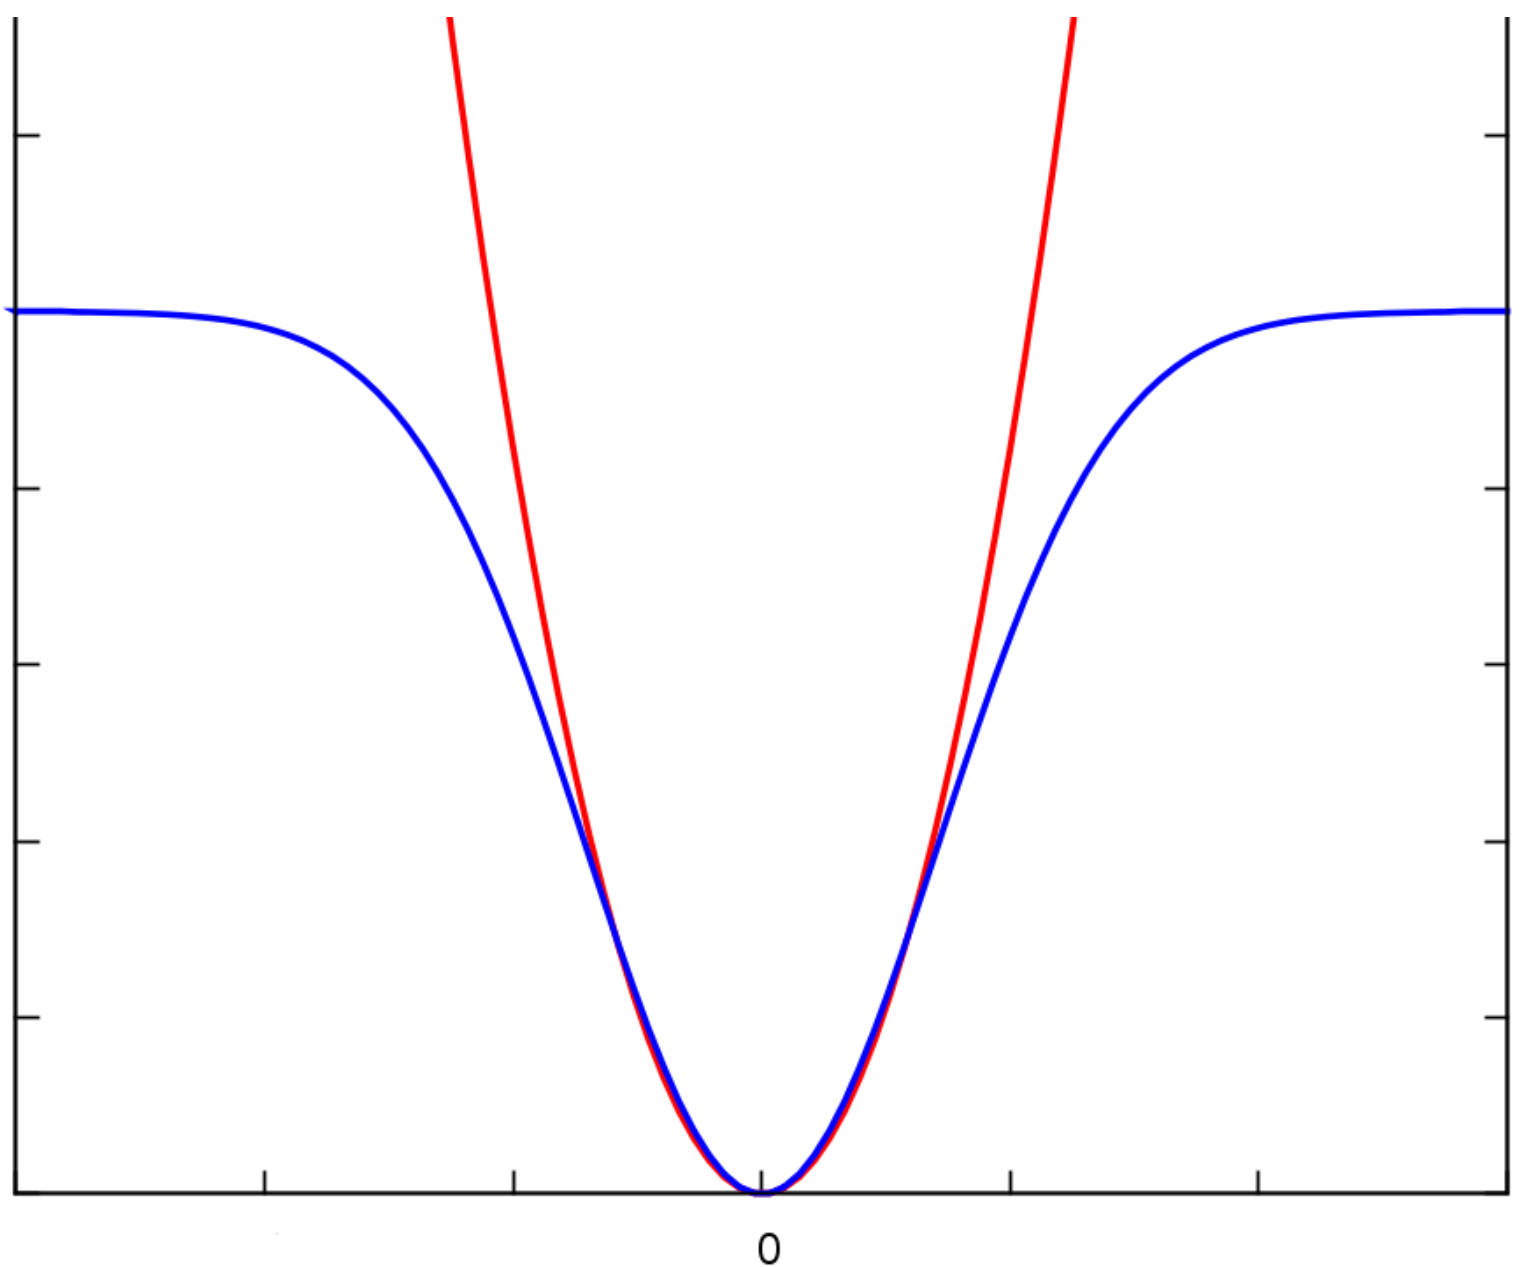
\includegraphics[scale=0.3]{images/WarchMethods.png}
\caption{L2 error (red) versus the robust Welsh's function (blue)}
\end{center}
\end{figure}


\paragraph{Gauss Error Function} \mbox{}
\par In statistics, for nonnegative values of $x$, the error function has the following interpretation: for a random variable $Y$ that is normally distributed with mean $0$ and variance $1/2$, $erf(x)$ describes the probability of $Y$ falling in the range $[-x, x]$.
\begin{equation}
erf(x)=\frac{1}{\sqrt{\pi}} \int_{-x}^{x} e^{-t^2} dt = \frac{2}{\sqrt{\pi}} \int_0^{x} e^{-t^2}dt
\end{equation}
Approximation gauss error function with elementary functions:
\begin{equation}
erf(x)=1-\frac{1}{(1+a_1x+a_2x^2+a_3x^3+a_4x^4)^4} \hspace{10pt} {\color{red}x \geq 0} \hspace{10pt} (\textbf{maximum error:} 5×10^{-4})
\end{equation}
\par Where $a_1=0.278393, a_2=0.230389, a_3=0.000972, a_4=0.078108$

\begin{figure}[H]
\begin{center}
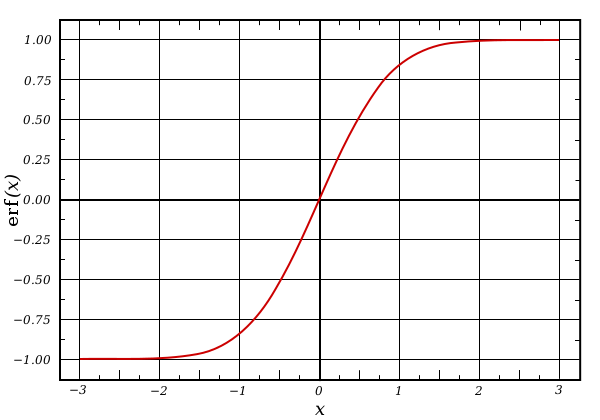
\includegraphics[scale=0.5]{images/GaussErrorFunction.png}
\end{center}
\end{figure}

\begin{thebibliography}{1}



\end{thebibliography}



\end{document}
